Pour aborder l'analyse de traces de sang, nous avons décidé d'utiliser le modèle Resnet 50~\cite{ResNet} pré-entraîné sur ImageNet selon certains poids indiqués dans la bibliographie~\cite{torchvision}, selon diverses approches. Nous avons utilisé la crossentropy pour notre fonction de coût, et Adam~\cite{adam} pour l'optimizer.

\subsection{ResNet linear probe}
Nous avons dans un premier temps retiré la dernière couche dense du modèle, qui était destinée à classifier sur 1000 catégories, puis effectuer du linear probing. Nous avons donc gelé tous les poids du Resnet et nous avons remplacé la dernière couche dense par 2 couches denses (qui elles sont apprenables) pour avoir une dernière couche dense à 18 neurones\footnote{la sortie correspond alors aux 18 modèles de taches de sang.}. La couche dense intermédiaire est de taille 64, et nous avons fixé un dropout à $0.1$. La Figure~\ref{fig:resnet} représente ce modèle linear probe ResNet. Les modèles utilisant le linear probing seront désignés par LP Resnet dans la suite.

\begin{figure}[ht]
    \centering
    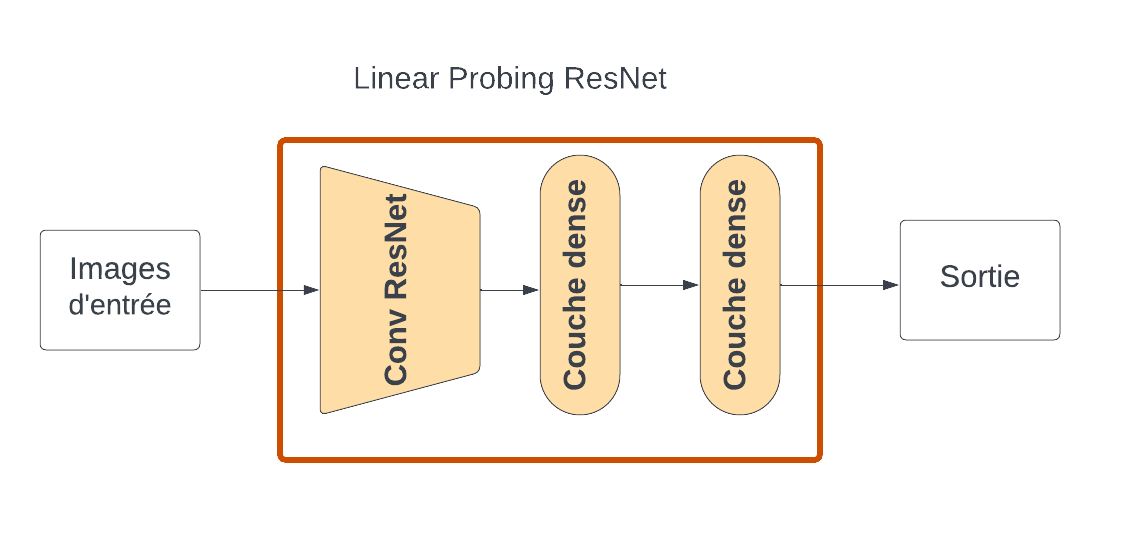
\includegraphics[width=0.7\linewidth]{../asset/Resnet.png}
    \caption{Schéma du modèle Resnet}
    \label{fig:resnet}
\end{figure}

\subsection{Réentraînement de tout le ResNet}
Nous avons également testé la méthode LP ResNet sans geler les poids de convolution du ResNet. Les modèles concernés par cette méthode seront désignés par "AWL ResNet" pour All weight learnable.

\subsection{Modèle Adversarial}

Un des points important pour la classification d'image est de pouvoir détecter la tache de sang et de la détacher du fond (background). Nous avons alors implémenté un entraînement adversarial. En plus du modèle ResNet, nous avons rajouté un modèle de MLP (Multilayer Perceptron) composé de deux couches fully connected layer qui prend en entrée la sortie de l'avant-dernière couche dense de notre Linear Probe ResNet, et prédit le background. Le but est d'alors de faire en sorte que le modèle ResNet ne possède pas d'informations sur le background de l'image dans son espace latent. La Figure~\ref{fig:resnet_adv} montre ces deux modèles. Nous appellerons cette approche "modèle Adversarial".

\begin{figure}[ht]
    \centering
    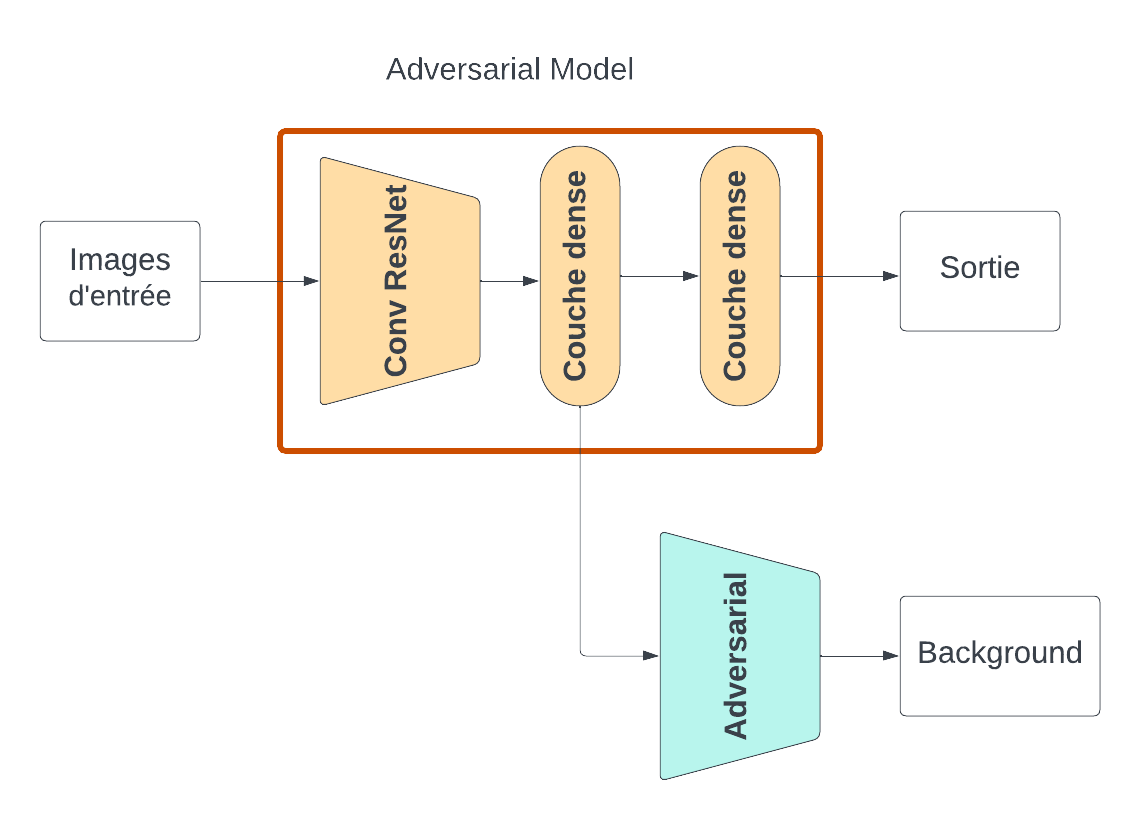
\includegraphics[width=0.7\linewidth]{../asset/Resnet_adv.png}
    \caption{Schéma du modèle Resnet adversarial}
    \label{fig:resnet_adv}
\end{figure}

Nous avons fait un entraînement adversarial pour entraîner les deux modèles simultanément. Nous avons utilisé la fonction de coût définie dans la Formule~\ref{eq: advloss}, où $CE_{tache}$ est la crossentropy entre la prédiction du modèle ResNet et la classe de la tache de sang, et $CE_{background}$ est la crossentropy de la prédiction du modèle adversarial et le background de l'image. Le paramètre $\alpha$ est un hyperparamètre que l'on va optimiser dans la section~\ref{sec: random search}.
\begin{equation}
    L_{adv} = \frac{CE_{tache}}{\alpha CE_{background}}
    \label{eq: advloss}
\end{equation}

La loss $L_{adv}$ est rétro-propagée dans le modèle ResNet tandis que la loss $CE_{background}$ est alors propagée dans le modèle adversarial.

\subsection{Fine-tune des modèles sur les données réelles}
Une fois que nous avons appris nos modèles LP ResNet et AWL ResNet sur les données de laboratoires, nous avons fine-tune ces modèles sur les données réelles (données issues de scène de crime). Nous avons appelé ces modèles respectivement FT LP Resnet et FT AWL ResNet.

Nous n'avons pas pu fine-tune le modèle Adversarial, car les taches de sang ne sont pas sur les fonds unis, et par conséquent, il n'est pas possible de fine-tune le modèle prédicteur de background sur ces données.
